\documentclass[12pt]{article}
% \usepackage[portuguese]{babel}

\usepackage{sbc-template}

\usepackage{graphicx,url}
\usepackage{listings}
\usepackage{xcolor}
 
\definecolor{codegreen}{rgb}{0,0.6,0}
\definecolor{codegray}{rgb}{0.5,0.5,0.5}
\definecolor{codepurple}{rgb}{0.58,0,0.82}
\definecolor{backcolour}{rgb}{0.95,0.95,0.92}
 
\lstdefinestyle{mystyle}{
    backgroundcolor=\color{backcolour},   
    commentstyle=\color{codegreen},
    keywordstyle=\color{magenta},
    numberstyle=\tiny\color{codegray},
    stringstyle=\color{codepurple},
    basicstyle=\ttfamily\footnotesize,
    breakatwhitespace=false,         
    breaklines=true,                 
    captionpos=b,                    
    keepspaces=true,                 
    numbers=left,                    
    numbersep=5pt,                  
    showspaces=false,                
    showstringspaces=false,
    showtabs=false,                  
    tabsize=2
}
\usepackage{float}
 
\lstset{style=mystyle}

\usepackage[brazil]{babel}   
\usepackage[utf8]{inputenc}  

     
\sloppy

\title{Gerenciamento de Redes:\\ Monitoramento com Nagios}

\author{
Ian Gustavo Alves Pessoa\inst{1}, Levi da Silva Lima\inst{2}, William Azevedo da Silva\inst{3}, \\Daniel Akio Chen\inst{4} }


\address{Núcleo de Computação -- Universidade do Estado do Amazonas
  (UEA)\\
  Manaus -- AM -- Brazil
  \email{\{igaps.eng17, ldsl.eng16, wads.eng16, dac.eng17\}@uea.edu.br}
}

\begin{document} 

\maketitle

\begin{abstract}
    This work aims to make a study on the COVID-19 case database in the minicipio de manaus taking into account a period from 01/04/2020 to 07/31/2020. For this, the development tools present for Python were used with the help of Google Colab development environment, which gathers devices for analyzing large amounts of data. The auxiliary tools used were pyplot, plotly, pandas and spicy which were used for specific calculations, data handling and graph plotting.
\end{abstract}
     
\begin{resumo} 
   Este trabalho tem por objetivo fazer um estudo sobre a base de dados de casos de COVID-19 no município de Manaus levando em consideração um período que vai de  01/04/2020 à 31/07/2020. Para tal foram utilizadas as ferramentas de desenvolvimento presentes para Python  com o auxilio do ambiente de desenvolvimento Google Colab que reúne aparatos para analise de grande quantidade de dados. As ferramentas auxiliares utilizadas foram pyplot, plotly, pandas e spicy para cálculos específicos, manipulação de dados e plote de gráficos.
\end{resumo}

\section{Fundamentação Teórica}

\textit{Python} é uma linguagem de programação de alto nível,interpretada, de \textit{script}, imperativa, orientada a objetos, funcional, de tipagem dinâmica e forte. Foi lançada por Guido van Rossum em 1991. Atualmente possui um modelo de desenvolvimento comunitário, aberto e gerenciado pela organização sem fins lucrativos Python Software Foundation. Apesar de várias partes da linguagem possuírem padrões e especificações formais, a linguagem como um todo não é formalmente especificada.

Dentre as diversas bibliotecas presentes no \textit{python}, para esse projeto vale ressaltar: \textit{pandas}, \textit{matplotlib}, \textit{plotly}, \textit{math}, \textit{scipy}, \textit{datetime} que são usadas para fazer cálculos específicos e também para construir imagens e referencias interativas em forma de gráficos sobre um conjunto de informações.

Por fim o ambiente de codificação Google Colab que se reuniu como um coletivo em 1977, usando pela primeira vez o nome Green Corporation, e inicialmente recebeu uma bolsa \textit{nea workshop} através do Center for New Art Activities, Inc. Um pequeno sem fins lucrativos formado em 1974 que reúne todas essas ferramentas de forma a permitir o uso sem qualquer restrição por parte dos usuários

\section{Desenvolvimento}
% ---------------- begin --------------------

\subsection{Visão de Casos Confirmados}

No que tange as definições iniciais relacionadas ao \textit{dataset} de casos de Covid-19 em Manaus é importante ressaltar algumas considerações iniciais sobre os dados, levando em consideração que a data de coleta da base de dados para estudo foi no dia 31/07/2020. Sendo assim destaca-se:

\begin{itemize}
    \item Cada exemplo da base de dados é descrito por 36 valores distintos, sendo eles: '\_idade',
    '\_faixa etária', '\_sexo', '\_bairro', '\_classificacao', '\_comorb\_renal', '\_comorb\_diabetes',
    '\_comorb\_imuno', '\_comorb\_cardio', '\_conclusao', '\_dt\_notificacao', '\_taxa',
    '\_dt\_evolucao',
    '\_raca', '\_dt\_sintomas', '\_criterio', '\_tipo\_teste', '\_sintoma\_garganta',
    '\_sintoma\_dispneia',
    '\_sintoma\_febre', '\_sintoma\_tosse', '\_sintoma\_outros', '\_etnia', '\_profiss\_saude',
    '\_srag',
    '\_se\_notificacao', '\_distrito', '\_bairro\_mapa', '\_comorb\_respiratoria',
    '\_comorb\_cromossomica',
    '\_comorb\_hepatica', '\_comorb\_neurologica', '\_comorb\_hemato', '\_comorb\_obessidade',
    '\_origem', '\_evolução'
    \item Segundo a base de dados, em Manaus há cumulativamente 36671 casos confirmados
    \item O período de tempo que a base de dados abrange vai de 01/04/2020 a 31/07/2020
\end{itemize}

Para uma visualização mais concreta e precisa, foi feita uma limpeza na base de dados de casos de COVID-19, entre elas foi feita a remoção das colunas de : \_comorb\_renal', '\_comorb\_diabetes', '\_comorb\_imuno', 
'\_comorb\_cardio', '\_comorb\_respiratoria', '\_comorb\_cromossomica', 
'\_comorb\_hepatica', '\_comorb\_neurologica', '\_comorb\_hemato', '\_comorb\_obessidade', '\_sintoma\_garganta', '\_sintoma\_dispneia', '\_sintoma\_febre', '\_sintoma\_tosse', '\_sintoma\_outros', '\_etnia', '\_raca', '\_profiss\_saude', '\_dt\_evolucao', '\_dt\_sintomas', '\_origem', '\_evolução', '\_criterio'.

\subsubsection{Análise exploratória}
Com a base de dados limpa, pode-se responder alguns questionamentos sobre a estrutura e a disposição dos dados. Apos a limpeza e organização da base de dados é possível se afirmar que do total restaram 36671 exemplos sendo estes descritos por 13 atributos cada, implicando assim em uma queda aproximada de $65\%$ com relação a quantidade original de dados o que leva a concluir que havia uma quantia considerável de dados ruidosos. Sendo assim, a partir desse ponto sempre que for mencionado base de dados essa já corresponde aos dados consistentes filtrados. 

Para se ter uma sensibilidade percentual dentre os casos de COVID-19 dados como recuperados e não recuperados, foi feita uma análise sobre a base de dados obtendo-se o resultado de que $30.72\%$ de todos os casos presentes foram dados como recuperados. Vale ressaltar que a maior quantidade de casos acometidos de COVID-19 foram em mulheres. A Figura ~\ref{fig:uc} demonstra graficamente o resultado.
\begin{figure}[H]
\centering
    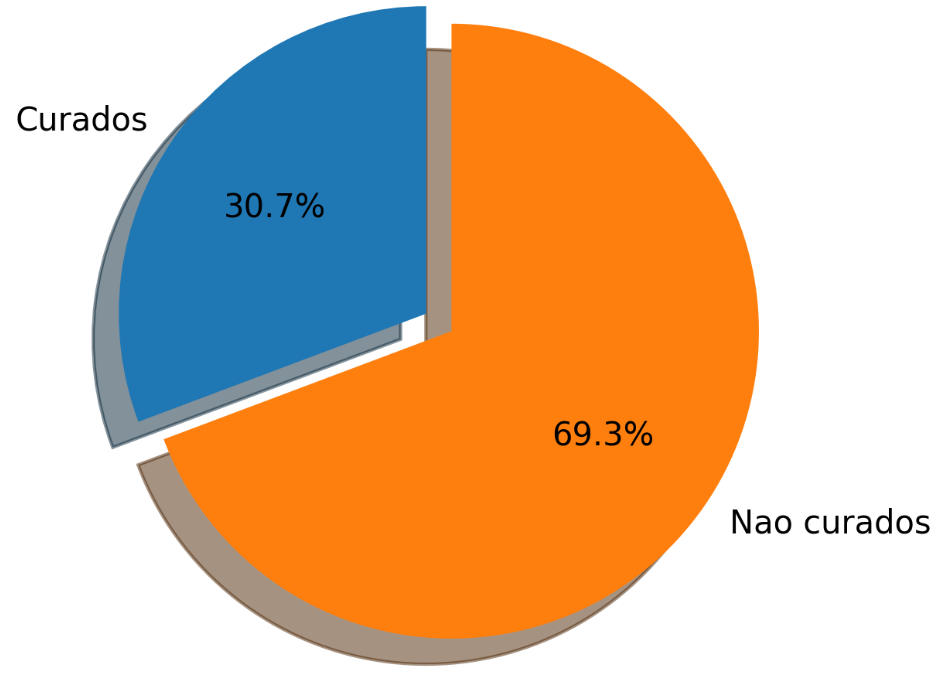
\includegraphics[width=6.5cm]{img/recuperados.png}
    \caption{Gráfico de relação percentual entre recuperados e não recuperados}
    \label{fig:uc} % Toda figura tem que ter um label diferente
\end{figure}

Facilmente percebe-se que não basta um simples calculo percentual para se ter um conhecimento solido sobre os dados, então para um melhor conhecimento sobre a disposição das informações foi feito um estudo estatístico, sobre a idade dos indivíduos que contraíram COVID-19, que envolvem a media e o desvio padrão pois eles permitem ter, respectivamente, uma visão geral da base de dados e também ter uma noção do grau de variação entre o conjunto de dados. Sendo assim, obteve-se o valor de $43.0$ para media que indica que no geral as pessoas que contraíram a doença tem 43 anos e $16.92$ para o desvio padrão que mostra que os valores podem se diferenciar da média por 17 anos indicando um possível intervalo de 26 a 60 anos para os indivíduos que contraíram a doença. Para concluir essa etapa da análise vale ressaltar qual é o verdadeiro intervalo de idade entre os indivíduos listados na base de dados, sendo assim é possível indicar que o individuo mais velho a contrair a doença tinha 120 anos e o mais novo 0 anos (criança recém nascida).

Partindo agora para um estudo que leva mais em consideração a disposição espacial das pessoas que moram em Manaus vale citar que o bairro com maior incidência de casos confirmados foi o bairro CIDADE NOVA com um total de 2008 casos e em contra partida a isso, os 3 bairros com maior quantidade de pessoas dadas como RECUPERADAS foram: CIDADE NOVA, FLORES e CENTRO. Dentre os casos confirmados há ainda aqueles que não fizeram nenhum tipo de exame, no entanto, dentre os que fizeram constata-se que estes foram de 5 tipos diferentes, sendo eles: ECLIA IgG, ELISA IgM, RT-PCR, TESTE RÁPIDO - ANTICORPO, TESTE RÁPIDO - ANTÍGENO. Para se ter uma maior sensibilização sobre os testes feitos tanto de forma quantitativa como percentual observe os gráficos na Figuras~\ref{fig:uc1} e na Figura~\ref{fig:uc2} que mostram a disposição dessas informações.
\begin{figure}[!ht]
\centering
    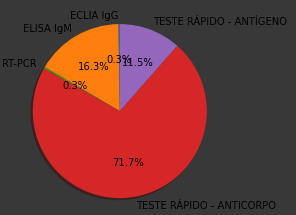
\includegraphics[width=9cm]{img/pizzar.png}
    \caption{Gráfico de percentual de cada teste que foi feito}
    \label{fig:uc1} % Toda figura tem que ter um label diferente
\end{figure}
\begin{figure}[!ht]
\centering
    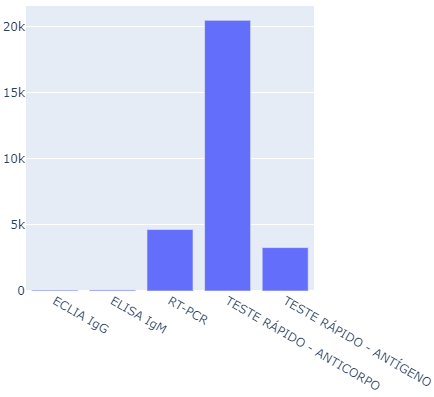
\includegraphics[width=10cm, height=8cm]{img/barrasteste.png}
    \caption{Gráfico de quantidade de cada teste que foi feito}
    \label{fig:uc2} % Toda figura tem que ter um label diferente
\end{figure}

Para finalizar essa etapa de análise exploratória dos dados é importante apontar que a taxa de letalidade foi de 5.5\%, que pode ser confirmado, o que indica um baixo valor percentual. Por fim o coeficiente de correlação de Pearson que visa medir as relações entre variáveis e o que elas representam foi de aproximadamente -0.3309 o que indica um correlação fraca e negativa ou inversa, indicando que as variáveis possuem baixa correlação. Como mostrado na Figura~\ref{fig:normal}, os casos possuem uma distribuição normal.

\begin{figure}[!ht]
\centering
    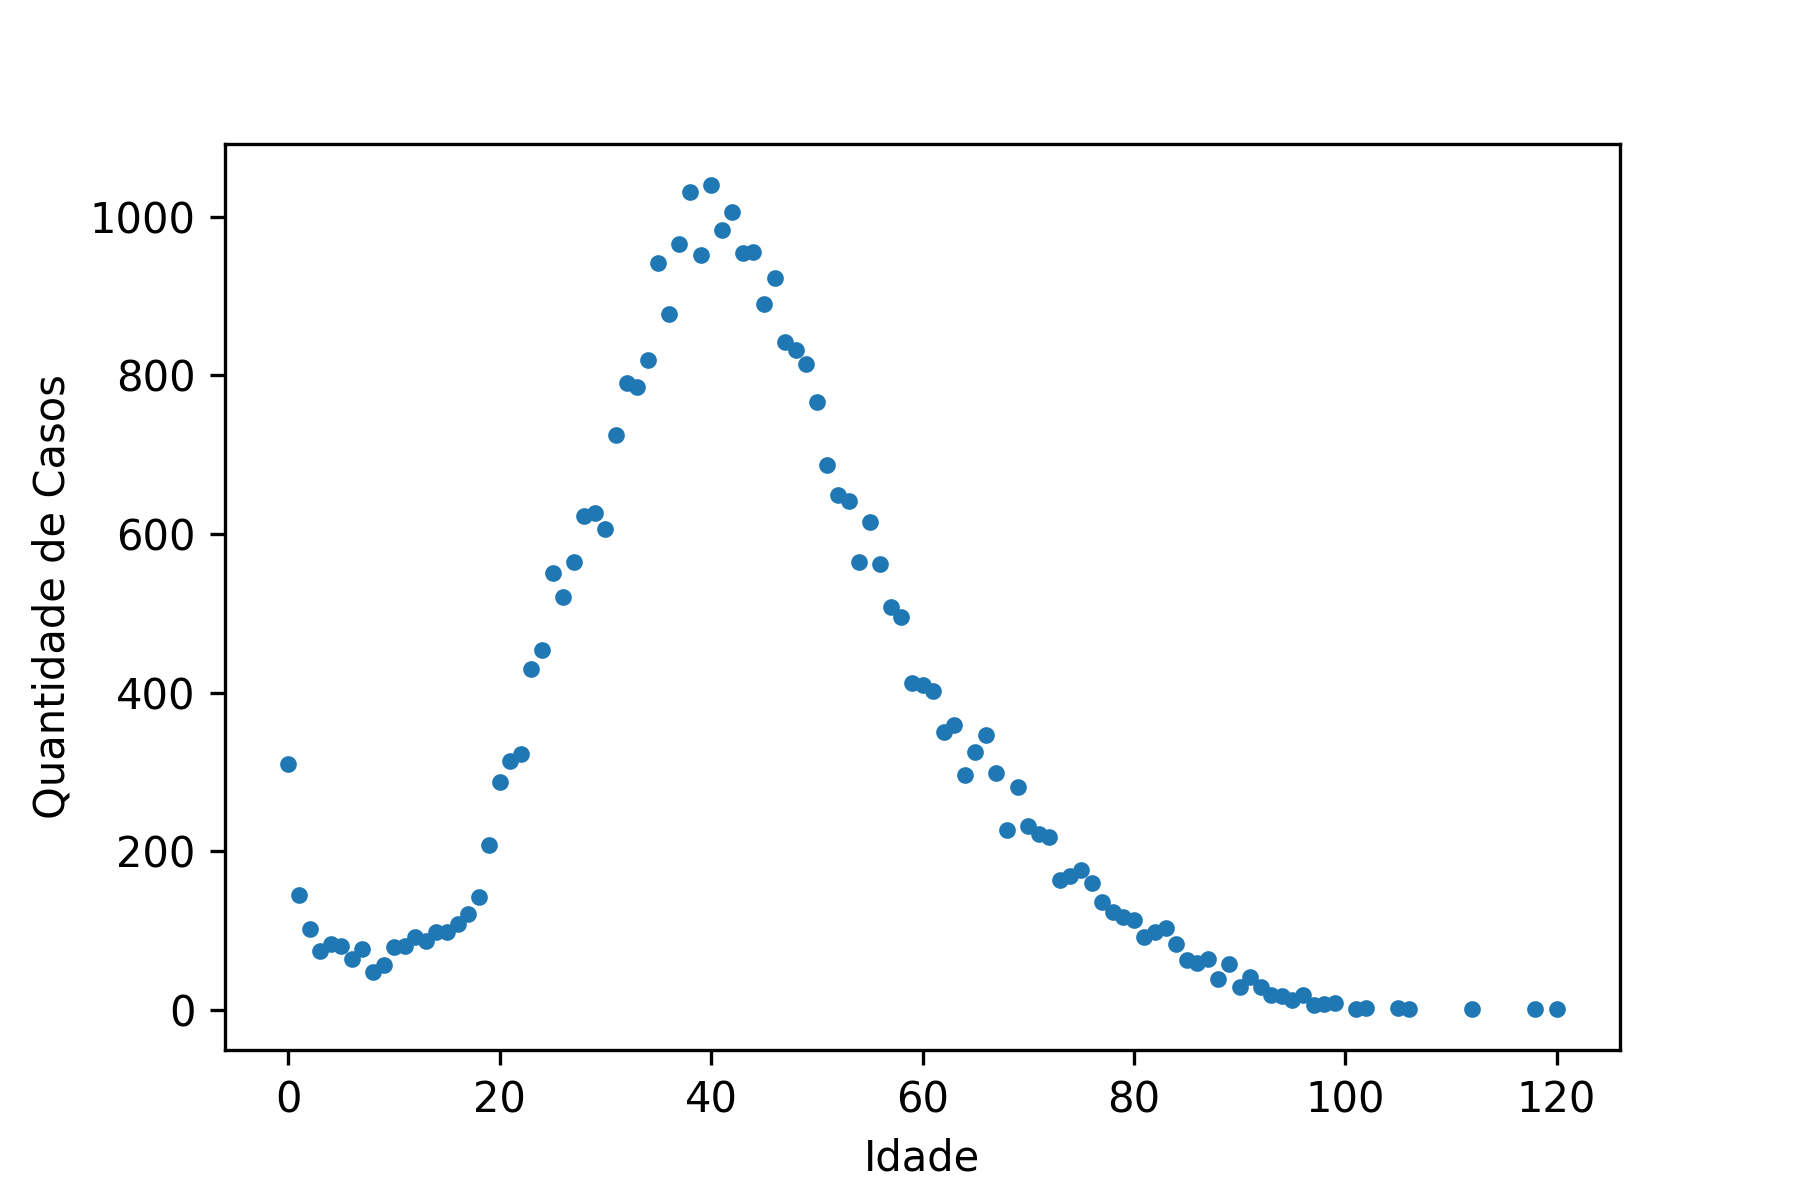
\includegraphics[width=10cm, height=8cm]{img/distribuicaoPorIdade.png}
    \caption{Gráfico de Distribuição por idade}
    \label{fig:normal} % Toda figura tem que ter um label diferente
\end{figure}


\subsection{Visualização de Dados}

Para se ter uma noção da disposição de casos de COVID-19 em Manaus, foi feito um estudo sobre a distribuição percentual de ocorrências, levando em consideração um agrupamento por bairros. Tendo isso em vista chegou-se ao seguinte gráfico da Figura~\ref{fig:uc3} que demonstra os 10 bairros com maior percentual de afetados (eixo x) e seus respectivos percentuais (eixo y), todos os demais bairros encontram-se juntos agrupados pelo rótulo de 'OUTROS'. Observa-se que existe certa uniformidade entre os bairros com maior índice de contaminados.
\begin{figure}[!ht]
\centering
    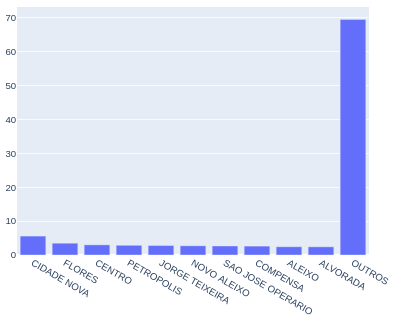
\includegraphics[width=6.8cm]{img/percentualPorBairro.png}
    \caption{Gráfico de percentual nos 10 bairros de maior ocorrência}
    \label{fig:uc3} % Toda figura tem que ter um label diferente
\end{figure}

Em adição a isso percebe-se que a variação entre os dados é de certa forma bem significante, para exemplificar isso foi feito o boxplot de casos confirmados por idade que estão mostrados na Figura~\ref{fig:uc4} e é perceptível a presença de \textit{outliers} (valores discrepantes) de forma expressiva na faixa 82 a 100 anos. Em conjunto com a Figura~\ref{fig:normal}, nota-se que as caudas da distribuição são largas e a dispersão  é baixa visto pelo tamanho da caixa representando os quartis. Os \textit{outliers} mostram que mesmo os mais idosos, acima de 100 anos e que são minoria, e as crianças mais novas, não foram privados do contágio, visto que de acordo com a Figura~\ref{fig:normal}, existe um pico para os recém nascidos.

\begin{figure}[!ht]
\centering
    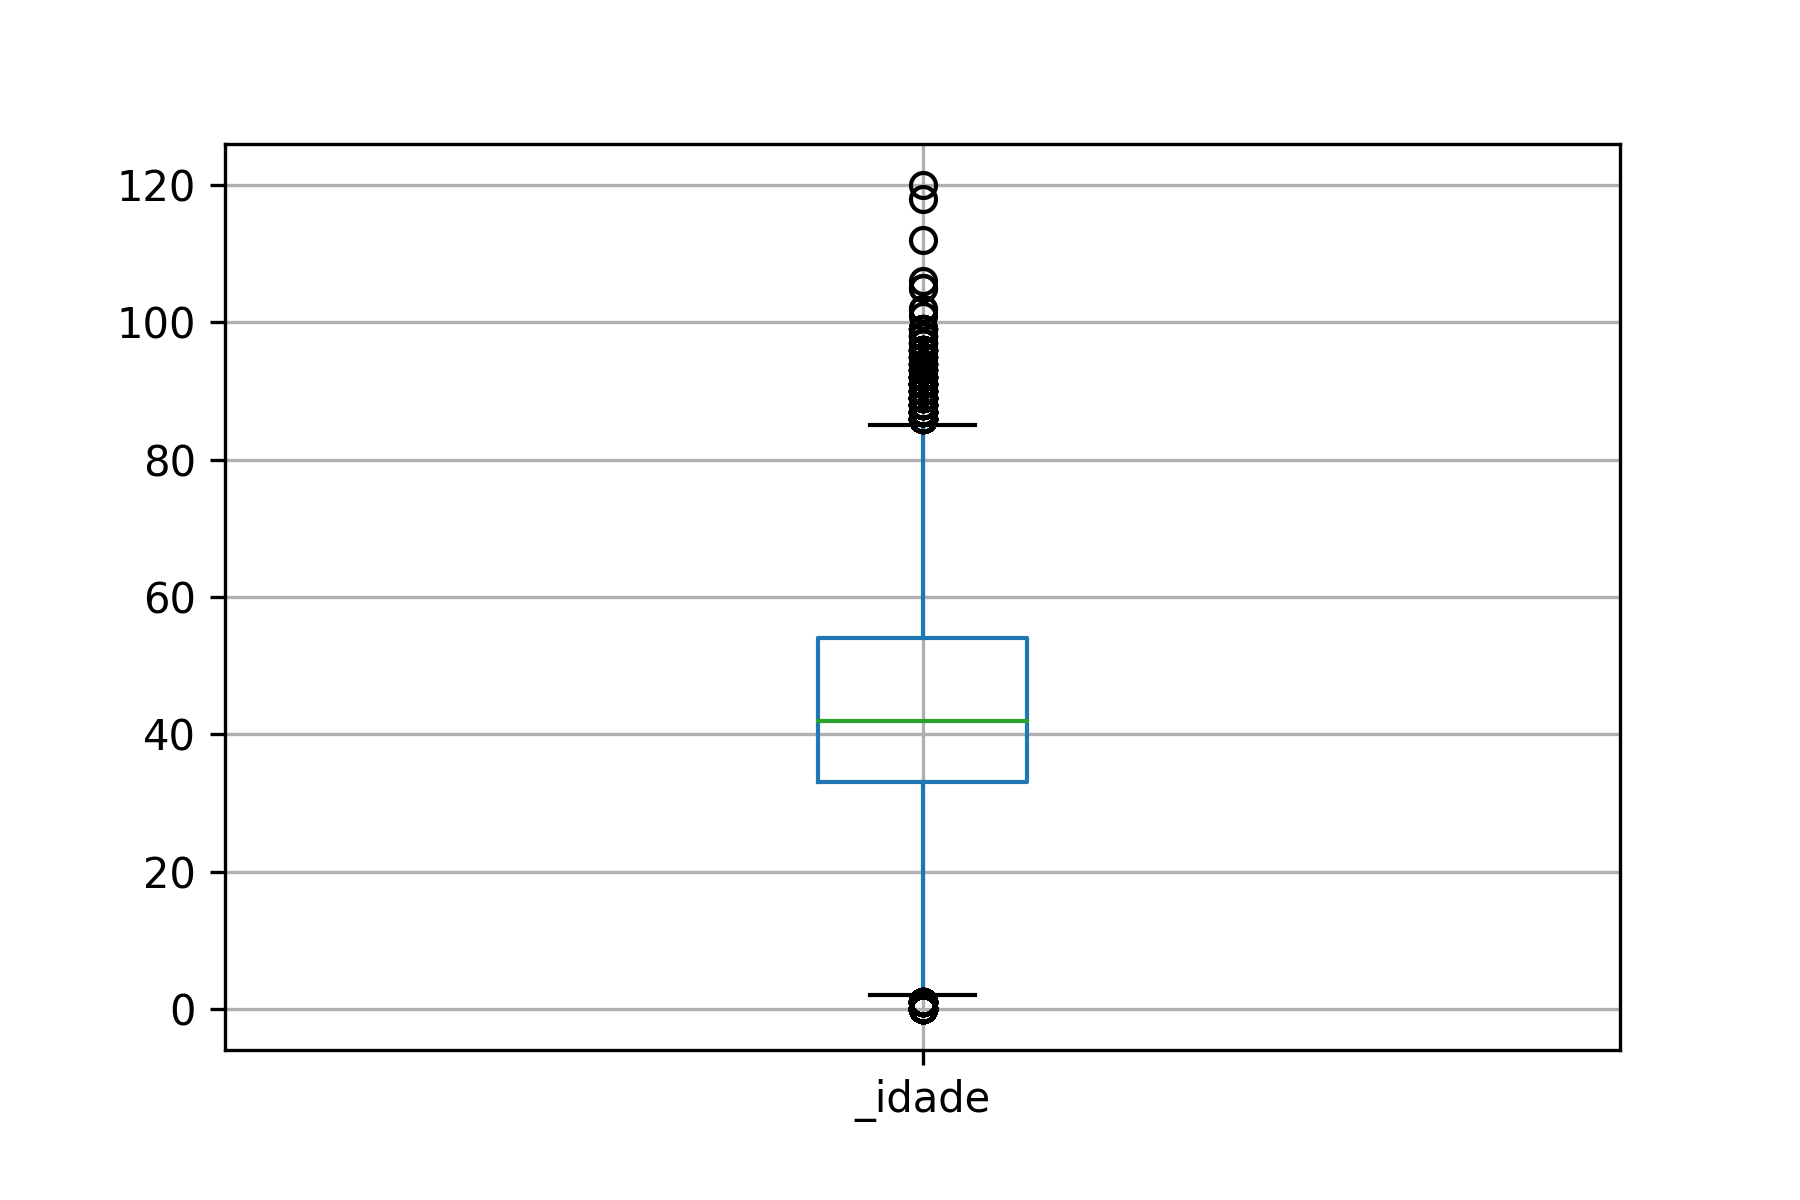
\includegraphics[width=8cm]{img/boxplot.png}
    \caption{Boxplot da idade dosS casos confirmados}
    \label{fig:uc4} % Toda figura tem que ter um label diferente
\end{figure}

Com um intuito de sensibilização do nível de contaminação do vírus, foi feito um gráfico, figura~\ref{fig:uc5}, que mostra a quantidade de novos casos confirmados nos últimos 10 dias contidos na base de dados, e também, para critério comparativo, foi feito um segundo gráfico similar ao da figura~\ref{fig:uc5} mas, levando em consideração a quantidade de pessoas recuperadas. O mesmo é representado pela figura~\ref{fig:uc6}. 

Como é possível constatar, a ocorrência de novos casos é muito mais recorrente que a de casos recuperados. Isso demonstra que a incidência do vírus tende a aumentar cada vez mais. É possível perceber também que todos os dias ouve novas notificações de casos enquanto de recuperados não.
\begin{figure}[!ht]
\centering
    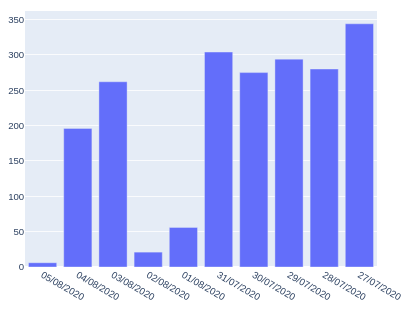
\includegraphics[width=8cm]{img/ultimos10dias.png}
    \caption{Número de novos casos por dia, considerando os 10 últimos dias existentes na base de dados}
    \label{fig:uc5} % Toda figura tem que ter um label diferente
\end{figure}
\begin{figure}[!ht]
\centering
    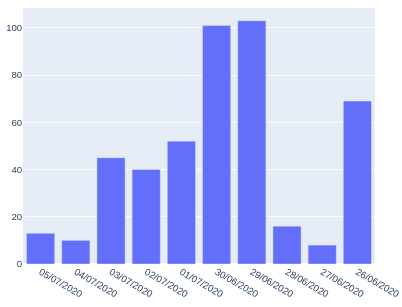
\includegraphics[width=8cm]{img/ultimos10diasConfirmados.png}
    \caption{Número de novos casos recuperados, considerando os 10 últimos dias existentes na base de dados}
    \label{fig:uc6} % Toda figura tem que ter um label diferente
\end{figure}

Visando analisar a quantidade de casos do vírus em relação as idades, foi feito um histograma, apresentado na figura 9, no qual é apresentado a relação Porcentagem x Faixa etária. Pelo histograma (figura 9), notamos que a quantidade de casos é baixa para as faixas etárias mais jovem e vai crescendo até 31 a 40 e 41 a 51. Depois disso, começa a cair, gerando assim, uma figura muito parecida com uma distribuição normal. Isso mostra que pessoas com idade de trabalho, provavelmente as que tiveram que sair de suas casas, ficaram mais vulneráveis ao vírus.

\begin{figure}[!ht]
\centering
    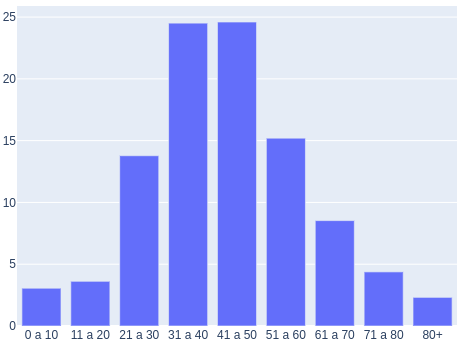
\includegraphics[width=8cm]{img/procentagemporidade.png}
    \caption{Histograma Porcentagem de Casos x Faixa etária}
    \label{fig:uc7} % Toda figura tem que ter um label diferente
\end{figure}

Para efeito demonstrativo o gráfico da figura~\ref{fig:uc8} mostra a curva da quantidade total de casos ao longo do tempo. Ao observar esse gráfico facilmente nota-se que a curva é ascendente com uma inclinação bem acentuada mas que por volta do mês 06 sofreu um pequeno desvio e seus valores começaram a diminuir (ainda sim é muito inclinada) semelhante a uma função logarítmica mas que ainda não chegou em seu ponto de equilíbrio e que mostra um possível aumento ainda nos meses seguintes.
\begin{figure}[!ht]
\centering
    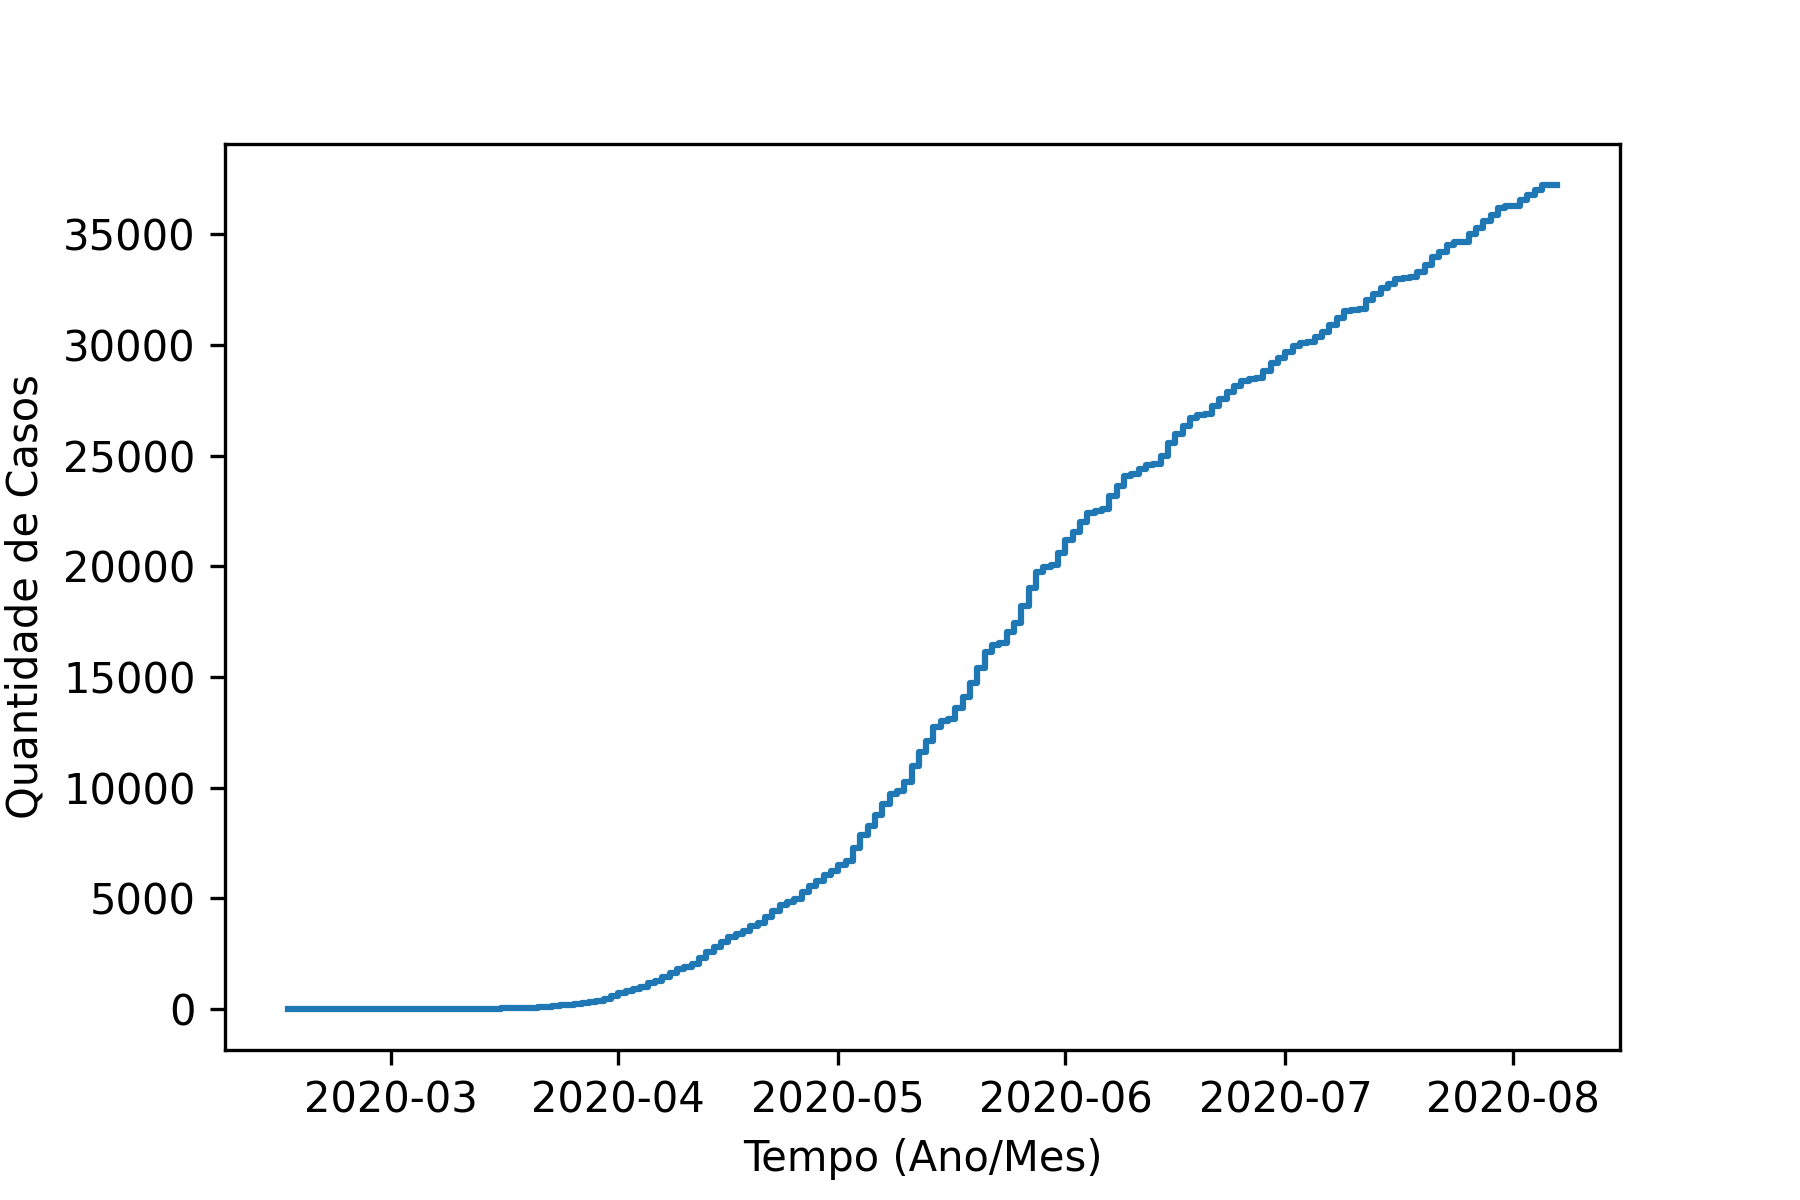
\includegraphics[width=9cm]{img/distribuicao2.6.png}
    \caption{Gráfico cumulativo de casos notificados ao longo do tempo}
    \label{fig:uc8} % Toda figura tem que ter um label diferente
\end{figure}

Já no gráfico~\ref{fig:uc9}, podemos ver um gráfico que denota a idade relacionada ao total de casos registrados para aquela certa idade, ou seja, usando os dados brutos. Comparando ao gráfico~\ref{fig:normal}, os dois são muito semelhantes, em ambos os gráficos, existe a tendência que os mais afetados são aqueles com aproximadamente 40 anos, mas também houve um pequeno pico nos recém-nascidos. Ou seja, o trabalhador médio que é em sua maioria na faixa de 40 anos estava mais sujeito a contaminação, nos extremos, a intensidade é menor porém ela é uniformemente distribuída e os recém nascidos foram bastante vulneráveis. 
\begin{figure}[!ht]
\centering
    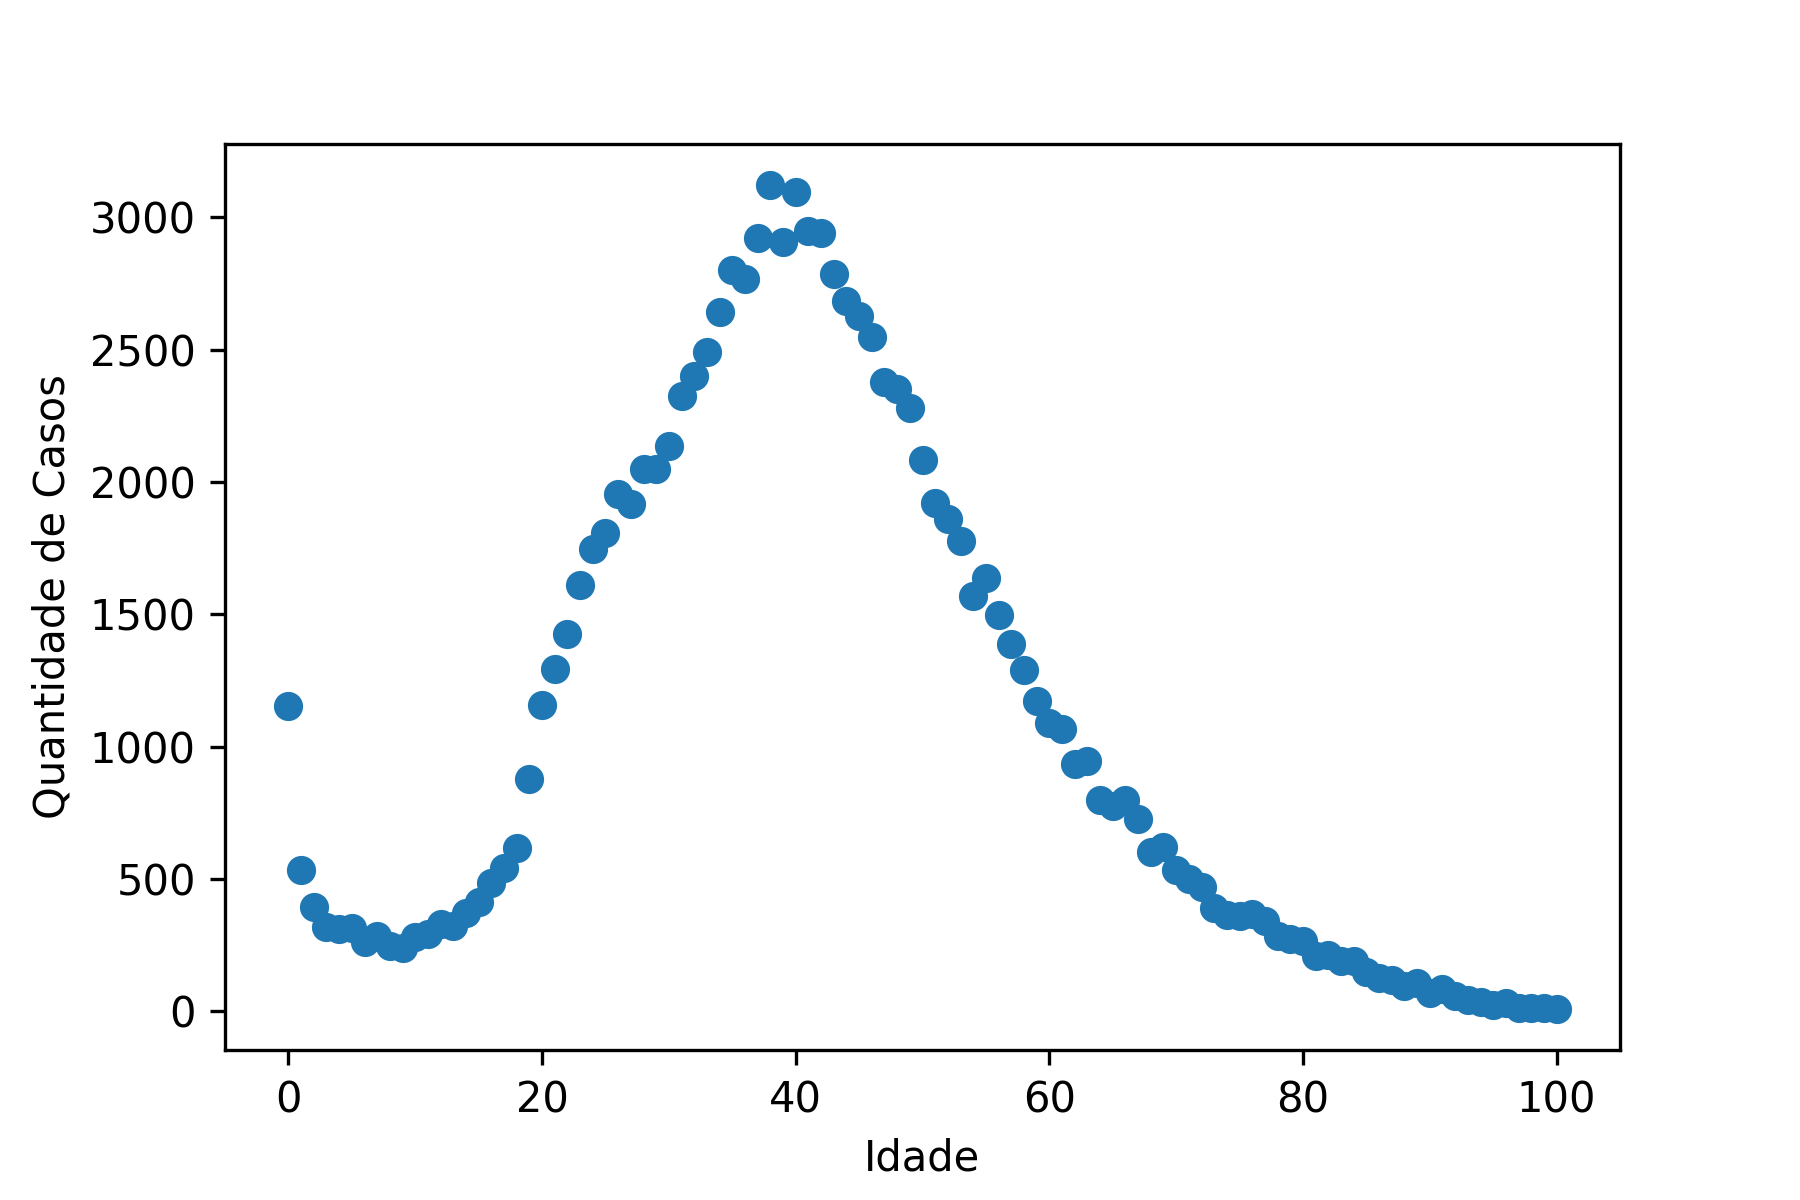
\includegraphics[width=9cm]{img/distribuicaoPorIdade2.7.png}
    \caption{Gráfico da idade versus o número total de casos registrados. Todos os casos registrados}
    \label{fig:uc9} % Toda figura tem que ter um label diferente
\end{figure}

\subsection{Tipos de Tarefas}

\subsubsection{Tarefa de Classificação mediante Aprendizado Supervisionado}

Uma tarefa de classificação que poderia ser usada é levar em consideração informações como: idade, comorbidades (diabetes, hipertensão), classificação (confirmado ou não) e a partir disso poder prever uma possível situação final para o individuo (recuperado ou óbito), para tanto pode-se utilizar algoritmos de aprendizado supervisionado como rede neural. Nesse contexto o atributo alvo para a rede neural seria 'conclusão' mostrando assim se o individuo se recuperou ou veio a óbito. Mas não basta apenas criar um modelo, treina-lo e por em pratica, é necessário avaliar a qualidade do modelo produzido e para isso há algumas métricas capazes de aferir tais características. Uma métrica que caberia a esse problema é o \textit{F1 Score} que é uma média harmônica entre precisão, ela é muito boa quando você possui um \textit{dataset} com classes desproporcionais (esse caso em particular é um desses), e o modelo não emite probabilidades (também se encaixa aqui). Obs: Isso não significa que não possa ser usada com modelos que emitem probabilidades, tudo depende do objetivo da tarefa de \textit{machine learning}.

\textit{Precision} também poderia ser usado nessa caso já que ele basicamente analisa o número de exemplos classificados como pertencentes a uma classe, que realmente são daquela classe (positivos verdadeiros) e divide pela soma entre este número, e o número de exemplos classificados nesta classe, mas que pertencem a outras (falsos positivos). O \textit{recall} que é bem similar ao que o \textit{precision} faz.

Para a validação dos dados pode-se utilizar métodos como \textit{Holdout}, \textit{Cross-Validation} e \textit{Leave-one-out} que permitem fazer a verificação do modelo de forma mais empírica.

\subsubsection{Tarefa de Regressão mediante Aprendizado Supervisionado}

Uma possível tarefa de regressão utilizando aprendizado supervisionado seria calcular a porcentagem de chance de uma pessoa recuperar-se, semelhante a questão anterior, porém, retornando a porcentagem de chance considerando um novo paciente. Os atributos preditores seriam os mesmo do método de classificação citado no exemplo a cima: idade, comorbidades, classificação (quanto a confirmação do vírus). 

Para a avaliação de desempenho, poderia ser utilizado a raiz quadrada do erro médio, que basicamente verifica o quão perto estão os dados da função gerada pela regressão.

\subsubsection{Tarefa de Aprendizado Não-Supervisionado}

No contexto de aprendizagem não supervisionada, poderia ser aplicado 
à este \textit{dataset}, uma clusterização dos dados, visando observar possíveis grupos de padrões (clusters) mostrando novas formas de observar os dados. Um possível algoritmo de clusterização a ser utilizado é o \textit{K-Means}, que agrupa os dados em \textit{K Clusters}. 



% ---------------- end -----------------------

\section{Conclusão}

Ao realizar este trabalho, foi possível aplicar vários conceitos sobre tratamento de dados, análise de dados (estatística) e exibição de dados (gráficos), aprendidos em sala de aula e durante estudos pessoais, o que certamente contribuiu para a formação profissional dos membros da equipe. 

Vale ressaltar que trabalhar com um problema atual e importante (COVID-19) foi estimulante para os membros da equipe, que ficaram gratificados em ver os resultados e comparar com os resultados divulgados pelos meios de comunicação.

\nocite{*}
\bibliographystyle{sbc}
\bibliography{sbc-template}

\end{document}
